\vspace{-3pt}
\section{Introduction}
\label{sec:introduction}

%\begin{figure}[h]
%	\centering
%	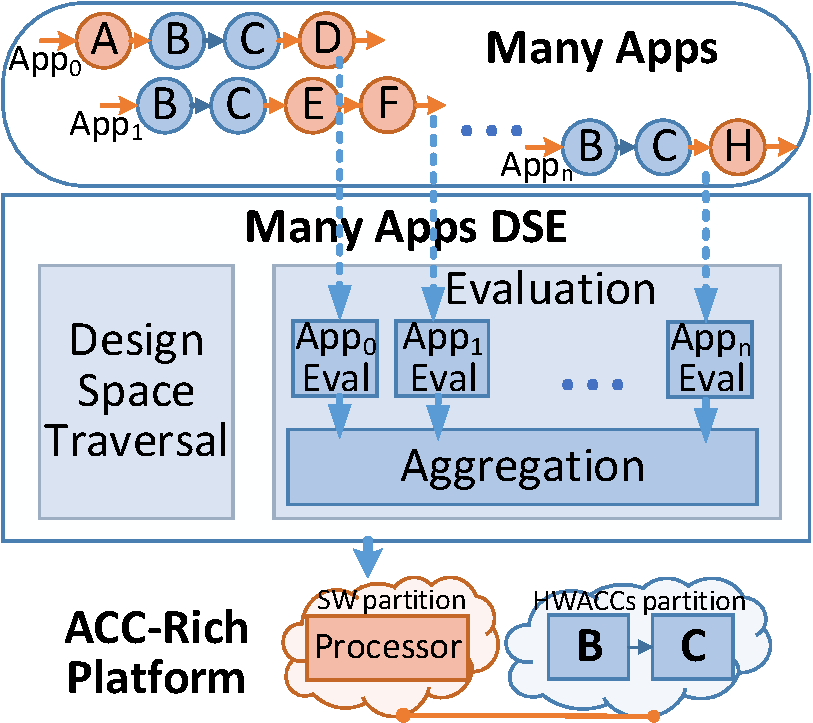
\includegraphics[width=.5\linewidth]{fig/MAARflow.pdf}
%	\caption{Promising Many Apps ACC-Rich Platform}
%	\label{fig:domainDSE}
%\end{figure}

%Tips: Mention Embedded or edge computing.

Using heterogeneous ACC-rich platforms~\cite{melpignano2012platform} that combine general-purpose processor(s) (SW) and custom ACCs (HW) is the primary approach for efficient, high-performance stream computing.
These platforms are typically designed targeting only a single application during allocation. Design Space Exploration (DSE) of one platform for each application is prohibitively expensive. In contrast to deep learning applications which often are computationally homogeneous and regular, such that a single monolithic accelerator can perform all linear algebraic computation required by deep learning algorithms, applications such as computer vision and software-defined radio demands a wide range of computationally intensive and functionality diverse heterogeneous accelerators (ACCs). The number of ACCs will increase dramatically, where individual ACCs are less monolithic but smaller and configurable. ACCs can be composed to accelerate larger kernels (or even applications).
%In contrast, platforms supporting many applications (e.g., FLP~\cite{tabkhi2016function}, Domain Platform~\cite{zhang2018ds}), that utilize similarities among applications, are promising to achieve flexibility to execute a set of applications efficiently.

\figref{fig:domainDSE} shows an example of a platform using $B$-$C$ ACCs to efficiently support many applications, which share $B$ and $C$ kernels. 
However, designing these platforms is a tremendous effort taking a vast amount of empiric knowledge into account. There is only little DSE methodology support for Many Applications ACC-Rich (MAAR) platforms because there is no existing evaluation to guide platform allocation for many applications. To feasibly allocate MAAR platforms, a MAAR DSE focusing on a set of applications, instead of individual applications in isolation, is needed.

\begin{figure}[ht]
  \centering
  \begin{minipage}[t]{0.24\textwidth}
    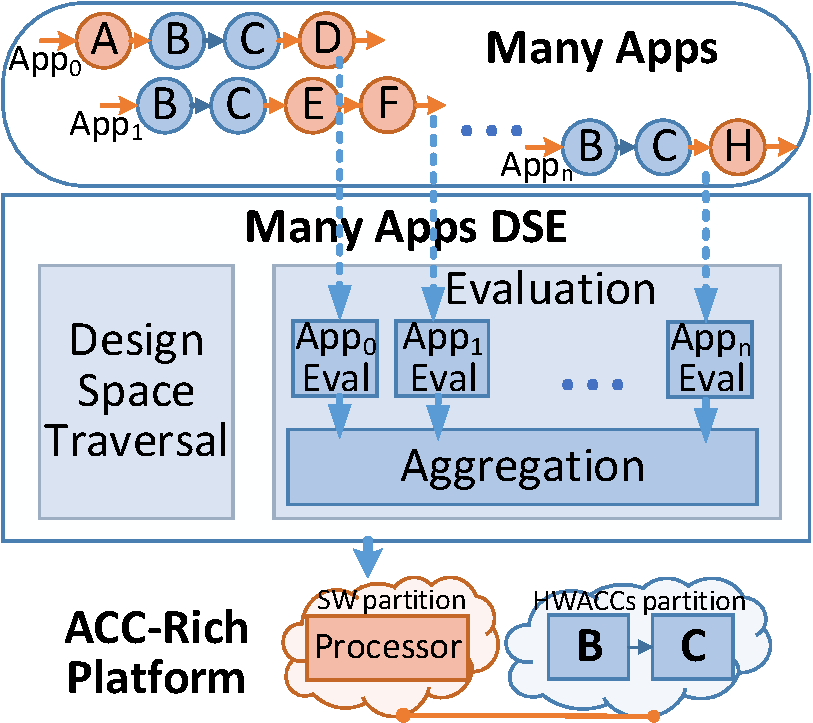
\includegraphics[width=.95\textwidth]{fig/MAARflow.pdf}
    \caption{Promising Many Apps ACC-Rich Platform}
    \label{fig:domainDSE}
  \end{minipage}%
  \hfill
  \begin{minipage}[t]{0.23\textwidth}
    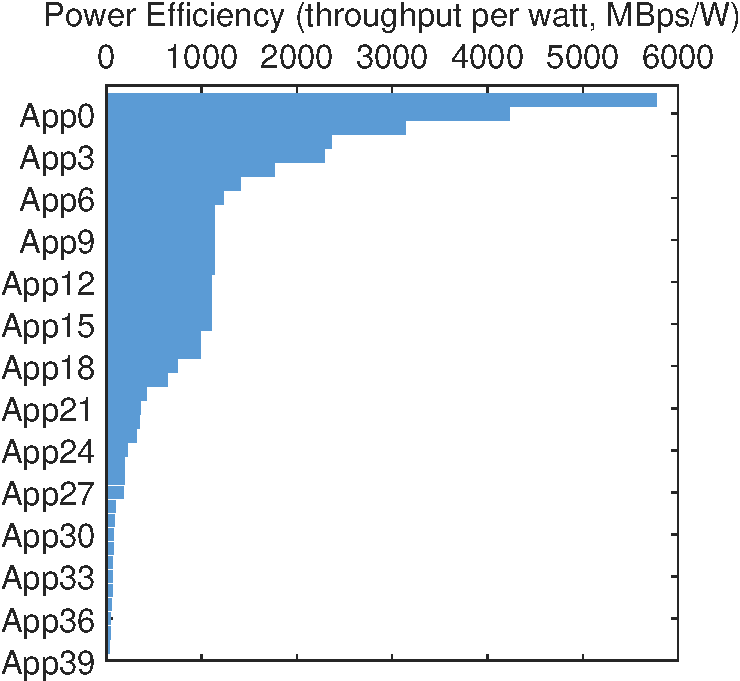
\includegraphics[width=1\textwidth]{fig/effIntro.pdf}
    \caption{Platform \newtext{Efficiency} for Applications}
	\label{fig:perf}
  \end{minipage}
\end{figure}

%\begin{figure}[h]
%	\centering
%	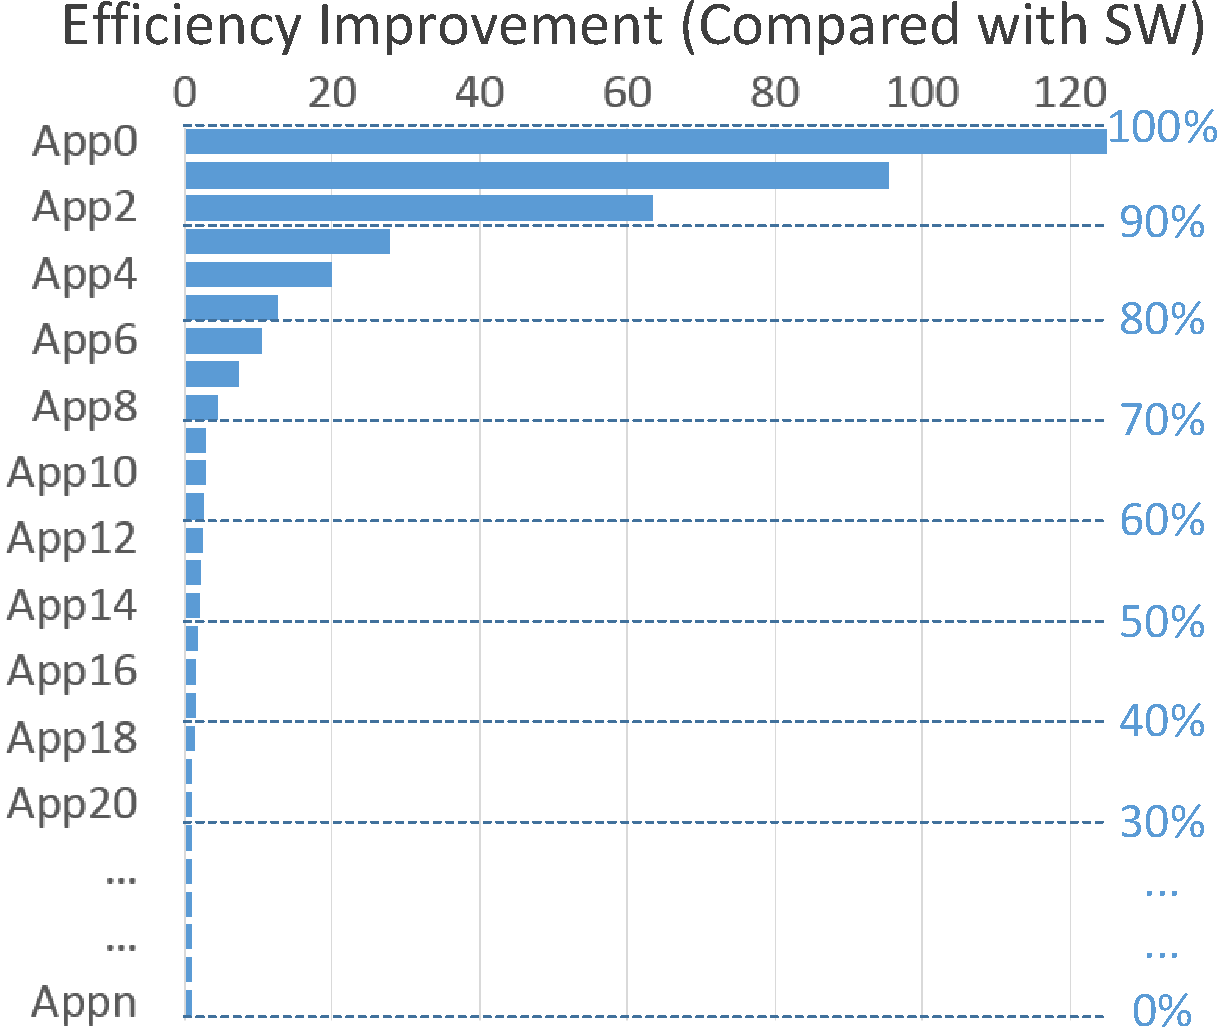
\includegraphics[width=.6\linewidth]{fig/Performance.pdf}
%	\caption{Domain Platform Efficiency Detail}
%	\label{fig:perf}
%\end{figure}

In \figref{fig:domainDSE}, many-application DSE has challenges in both design space traversal and a single design point (one platform) evaluation. Due to targeting to multiple applications, the design space of platform allocation is significantly larger than single application design, \newtext{and an efficient traversal is necessary.} 
Furthermore, the evaluation for many applications needs to have a fair focus on every application and provide an aggregated value to judge design quantitatively. Current platform evaluation primarily focuses the effects of the platform on one application in isolation. When moving to a set of applications, the simple average sum of all application performances is unfair. \figref{fig:perf} demonstrates the challenge of a MAAR platform evaluation. Because of the big variation among different applications' \newtext{efficiency} on the platform, the 10\% highest efficiency applications will dominate the DSE, if the evaluation simply sums all performances. As a result, the designed platform will not be efficient for many \newtext{low-efficiency} applications. To achieve a highly flexible and an efficient MAAR platform, a fair evaluation needs to aid the DSE in balancing the consideration of all applications.

%Hence, the traverse needs to be fast and efficient. 
%Besides high-speed request, 

%Unlike applications in a hand-composed benchmark, which balances contribution of each application to achieve a meaningful result, applications in a specified set of target applications have vastly different performances because of various parallelization and acceleration potential. 


This paper introduces MAAR DSE, guided by a platform evaluation for many applications with a balanced focus. To this end, the contributions of this paper are: (1) providing the flow of MAAR DSE, which is a combination of a heuristic traverse, elitist genetic algorithm (GA) and a fair evaluation for many applications; (2) defining relative efficiency of an application on a platform to have a normalized measure of improvement/achievement for different applications; (3) evaluating multiple methods to aggregate efficiency of many applications on a platform to quantitatively compare different platforms. The MAAR DSE fairly considers the contribution of many applications, and produces an efficient platform supporting all applications. In experiments using OpenVX applications, MAAR platforms achieve 3.09 times the average efficiency improvement of one application DSE (1appDSE), and 1.39 times the improvement of DSS, a previous domain platform DSE~\cite{zhang2018ds}. 
%With a budget of 12 ACCs, MAAR DSE's platform improves 67.5\% of applications by at least 3x, while 1appDSE only improves 15\% by 3x and DSS improves 42.5\% by 3x.

This paper is organized as follows: \secref{sec:related} summarizes the related works. \secref{sec:pre} introduces target ACC-rich platform and evaluation model for individual application. \secref{sec:eval} introduces MAAR DSE and fair MAAR platform evaluation methodology. \secref{sec:results} evaluates and analyzes the benefits of MAAR DSE with fair evaluation. Finally \secref{sec:conclusion} concludes this paper.


%\begin{figure}[h]
%    \centering
%    \begin{subfigure}[h]{.8\textwidth}
%        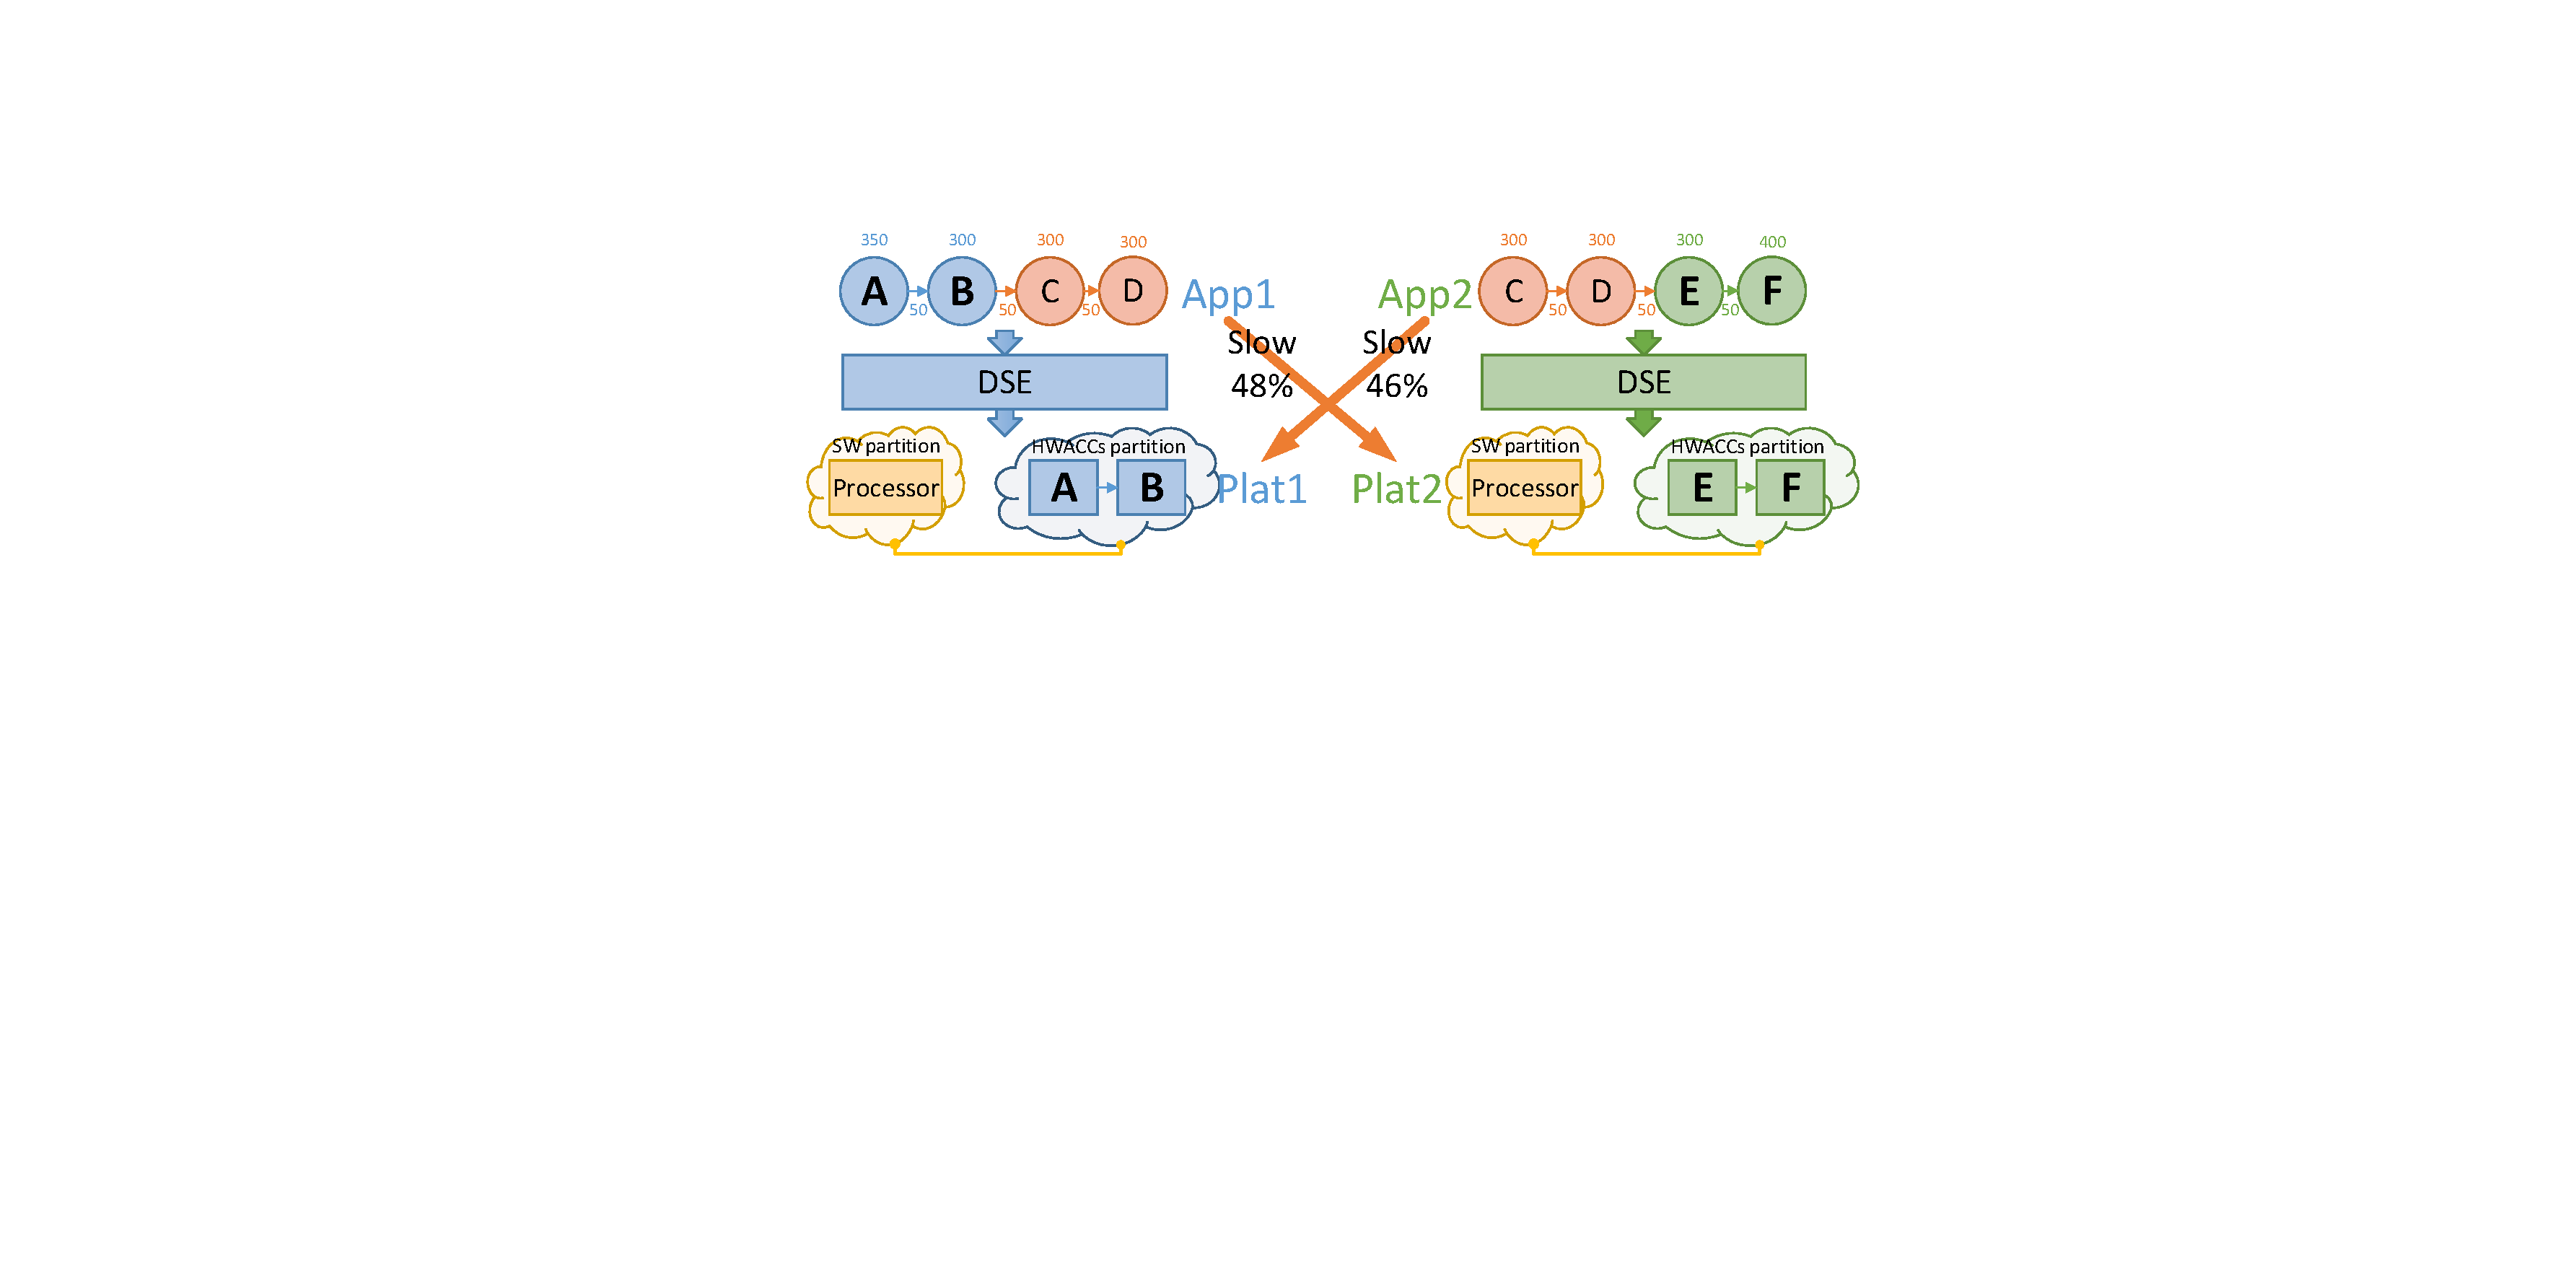
\includegraphics[h]{fig/pPlatApp.pdf}
%        \subcaption{App-Specific Platform]\label{fig:platApp}}
%    \end{subfigure}
%    \\
%    \begin{subfigure}[h]{.5\textwidth}
%        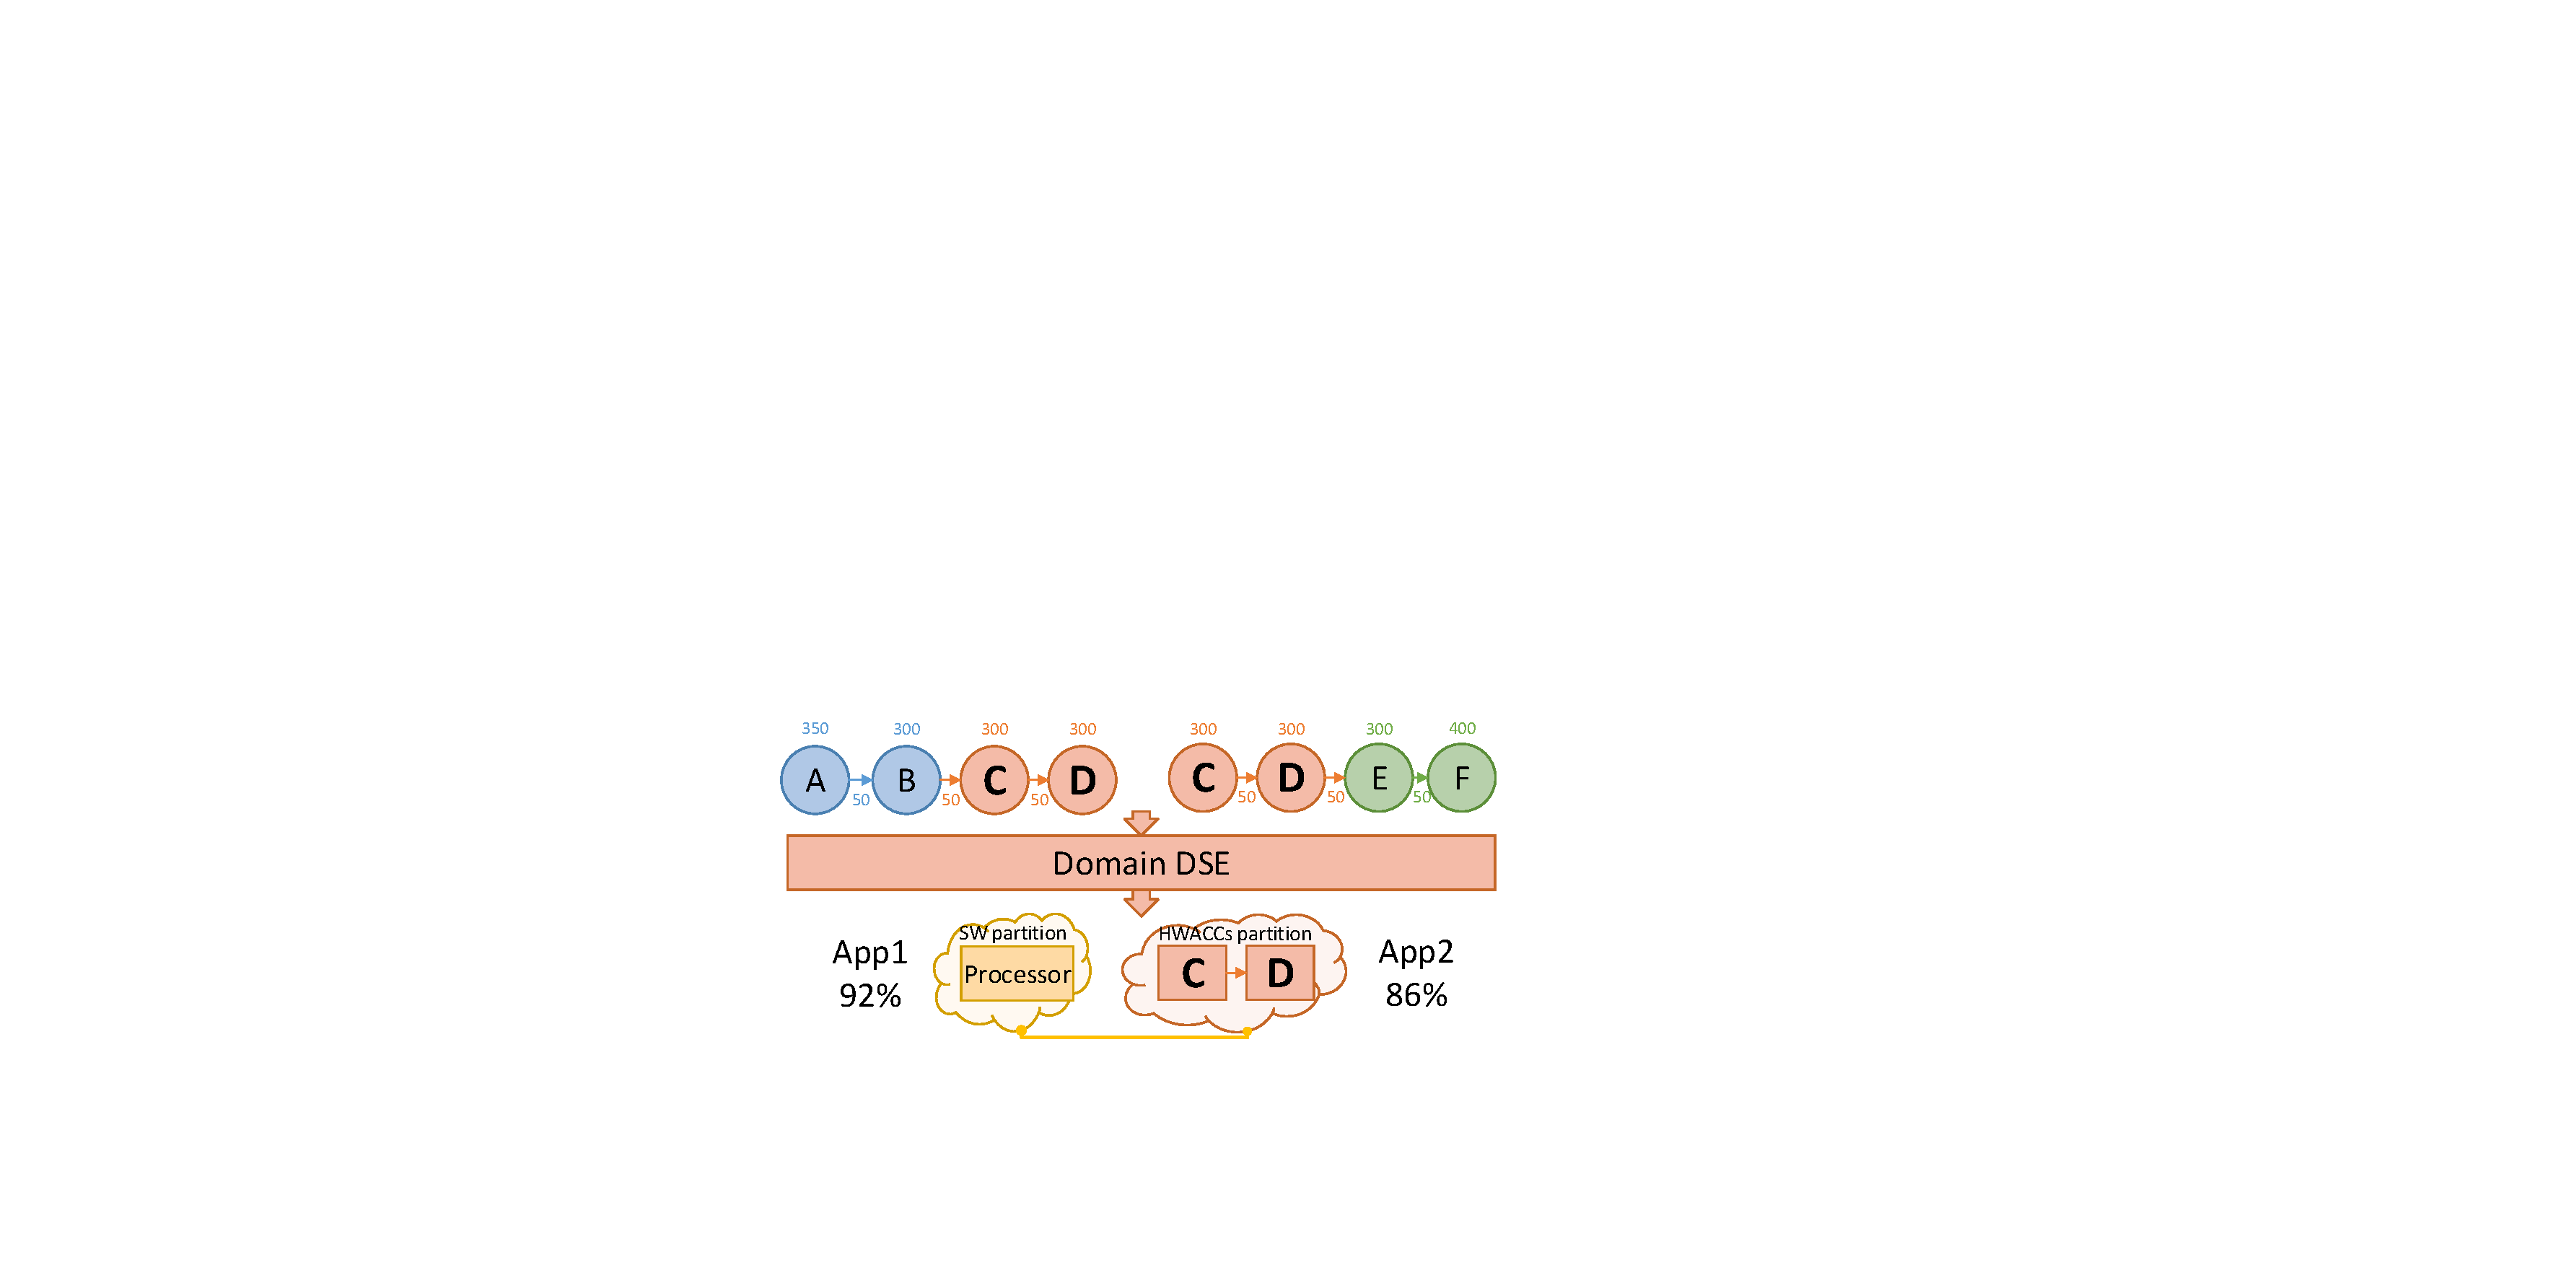
\includegraphics[h]{fig/pPlatDS.pdf}
%        \subcaption{Domain-Specific Platform]\label{fig:platDS}}
%    \end{subfigure}
%    \caption{Domain Platform: Penalty of Application Scope}
%    \label{fig:example}
%\end{figure}